%!TEX root = ../../main.tex

Sabe-se que algoritmos de AM necessitam de quantidade significantiva de dados, preferencialmente sem muitos ruídos, para serem utilizados de forma a obter um modelo que possua bom desempenho \cite{marsland}. Levando isto em conta e com vistas a adequar os dados disponíveis com a tarefa de aprendizado considerada, uma etapa de pré-processamento fez-se necessária, cujos passos são descritos a seguir.

Primeiramente foi necessário realizar a adaptação das imagens individuais para as imagens compostas, conforme apresentado anteriormente no esquema da Figura \ref{fig:esquema-solucao}. Para isto, foi feita a combinação de cada assinatura genuína de um autor com suas diferentes versões originais, produzindo uma nova imagem para cada caso, a qual associou-se o rótulo de autêntica. Após esta etapa, também foram combinados os exemplos genuínos com suas respectivas versões forjadas, aos quais foi associado o rótulo de forjado. Todas as imagens obtidas dessas combinações serão utilizadas como exemplos para o processo de treinamento, validação e teste do modelo proposto.

O processo de combinação das imagens de cada um dos exemplos foi realizado em três etapas. Na primeira etapa, ambas as imagens foram redimensionadas para um tamanho de $256 \times 256$ \emph{pixels}. Em seguida, as imagens foram concatenadas verticalmente com a intenção de formar uma única imagem de $256 \times 512$ \emph{pixels}. Por fim, a imagem resultante foi redimensionada novamente em um tamanho de $256 \times 256$ \emph{pixels} e transformada para um espaço de cores em escala de cinza, com a intenção de padronizar todos os exemplos.

Ao concluir a etapa anterior, realizou-se então nos exemplos autênticos, a partição \emph{holdout} previamente especificada. Para o exemplos forjados, percebeu-se que a existência de assinaturas realizadas por um mesmo autor forjador nos conjuntos da partição \emph{holdout}, levaria os modelos a prever, na etapa de teste e validação, dados muito parecidos com os encontrados no conjunto de treinamento. Sendo assim, para contornar este problema, a separação dos exemplos forjados foi baseada na quantidade de autores forjadores que cada assinatura autêntica possui e foi obtida segundo as seguintes regras:

\begin{itemize}
	\item Se uma assinatura autêntica possui apenas um autor forjador, todos os exemplos forjados referentes a esta assinatura vão para o conjunto de treinamento;
	\item Se uma assinatura autêntica possui quatro autores forjadores, as assinaturas de três desses autores irão para o conjunto de treinamento e as remanescentes, pertencentes a apenas um autor, irão para o conjunto de teste;
	\item Se uma assinatura autêntica possui cinco autores forjadores, as assinaturas de quatro desses autores irão para a etapa de treinamento e as remanescentes, pertencentes a apenas um autor, estarão presentes na etapa de teste;
	\item Se uma assinatura autêntica possui seis autores forjadores, as assinaturas de quatro desses autores irão para a etapa de treinamento e as assinaturas dos outros dois irão para a etapa de teste;
	\item Se uma assinatura possui trinta ou mais autores forjadores, as assinaturas de dez desses autores irão para o conjunto de teste, três desses autores serão utilizados para o conjunto de validação e as assinaturas restantes serão remanejadas para o conjunto de treinamento.
\end{itemize}

Os autores forjadores selecionados para estarem presentes em cada uma das partições foram selecionados de forma pseudoaleatória e, em todo o \emph{dataset}, não foram encontradas assinaturas que tenham sido forjadas por dois, três ou mais de seis e menos que trinta autores. Os dados de treinamento e validação, apesar da pequena desproporção encontrada entre as suas classes, foram dividos de modo a garantir o bom aprendizado das características dessas classes pelos modelos propostos. O conjunto de testes, por sua vez, apresenta uma característica desbalanceada. A Tabela \ref{tab:divisao-dados} apresenta a descrição destes dados, suas quantidades e divisões e a Figura \ref{fig:divisao-dados} auxilia na visualização da proporcionalidade nos diferentes conjuntos considerados.

\begin{table}[h!]
	\centering
	\caption{Quantitativo de exemplos por finalidade na tarefa de aprendizado considerada e classe.}
	\label{tab:divisao-dados}
	\begin{tabular}{c c c c}
		\toprule
		\textbf{Conjunto} & \textbf{Tipo de Exemplo} & \textbf{Quantidade de Dados} & \textbf{Proporção}\\
		\midrule
		\multirow{2}{*}{Treinamento} & Autêntico & 9.374 & $54\%$ \\
    & Forjado & 8.131 & $46\%$\\
     \midrule
		 \multirow{2}{*}{Validação} & Autêntico & 947 & $46\%$ \\
     & Forjado & 1.134 & $54\%$\\
		 \midrule
		 \multirow{2}{*}{Teste} & Autêntico & 6.119 & $73\%$ \\
     & Forjado & 2.257 & $27\%$\\
		\bottomrule
	\end{tabular}
\end{table}

\begin{figure}[h!]
\centering
\caption{Representação gráfica da proporção dos exemplos por classe e finalidade na tarefa de aprendizado considerada.}
\label{fig:divisao-dados}
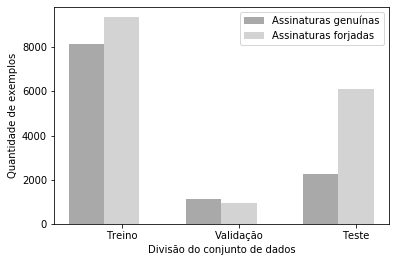
\includegraphics[width=0.7\textwidth]{imgs/divisao-dados}
\end{figure}

Ao serem fornecidas para treinamento pelas CNNs, todos os \emph{pixels} das imagens foram normalizados por meio de uma divisão por $255$, passando a residirem no intervalo $[0,1]$. Esta normalização é realizada em virtude das redes neurais que, em geral, aprendem mais eficientemente nestas condições \cite{chollet}.
